\documentclass{article}
\usepackage{polski}
\usepackage[utf8]{inputenc}
\usepackage{graphicx}
\usepackage{tabto}
\usepackage{hyperref}
%s\usepackage[margin=2.5cm]{geomtry}

\usepackage{graphicx}    % Pakiet pozwalający ,,wklejać'' grafikę...
\usepackage{subcaption}
\usepackage{amsmath,amssymb,amsfonts,amsthm,mathtools}
                               % Dołączamy zestaw różnych przydatnych znaczków ...
\DeclareMathOperator{\arccosh}{arccosh}
% dane autora
\author{Wiktor Pilarczyk}
\title{Warsztaty - W5 - SK\\\large{Prowadzący: Tomasz Wierzbicki}}
\date{\today}
% początek dokumentu
\begin{document}
\maketitle
\section{Część 1.}
\subsection{Ustawienia sieci}
Komendy użyte do konfiguracji sieci dla poszczególnej maszyny wirtualnej (po wcześniejszym sprawdzeniu adresów MAC w ustawieniach i interfejsów za pomocą 'ip link'):
\tabto{0.4cm}Virbian1:
\tabto{0.8cm}    sudo ip link set enp0s3 name enp0
\tabto{0.8cm}    sudo ip link set up dev enp0
\tabto{0.8cm}    sudo ip addr add dev enp0 192.168.0.1/24
\tabto{0.4cm}Virbian2:
\tabto{0.8cm}    sudo ip link set enp0s3 name enp0
\tabto{0.8cm}    sudo ip link set up dev enp0
\tabto{0.8cm}    sudo ip addr add dev enp0 192.168.0.2/24
\\
Po wszystkich instrukcjach warto sprawdzić czy się nie popełniono błedu komendą 'ip addr'.
\\
Komputery z tej samej sieci są osiągalne za pomocą komendy 'ping'.
\subsection{Adresy MAC maszyn}
\tabto{0.4cm}Virbian1:
\tabto{0.8cm}    08:00:27:e6:4a:13
\tabto{0.4cm}Virbian2:
\tabto{0.8cm}    08:00:27:77:1d:db
\\
\subsection{Ping 192.168.0.2}

\begin{figure}[!htb]
\centering
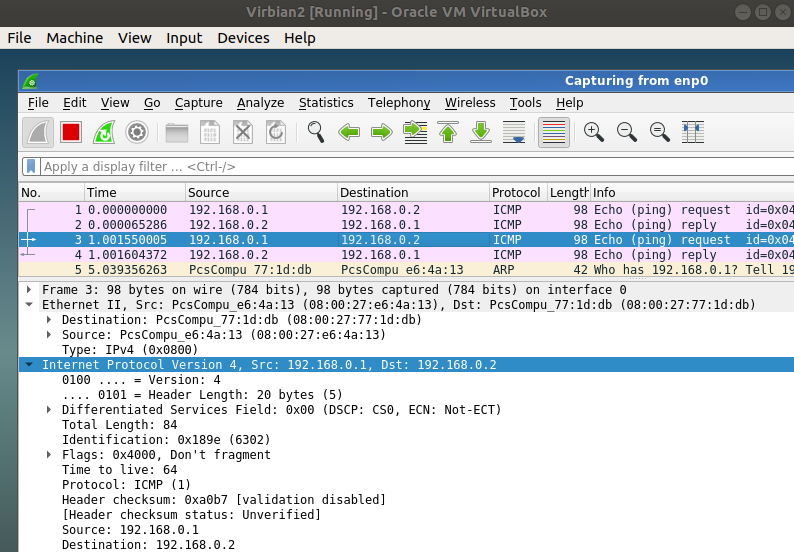
\includegraphics[width=11cm,height=5cm]{broadreq.png}
\caption{echo request}
\end{figure}

\begin{figure}[!htb]
\centering
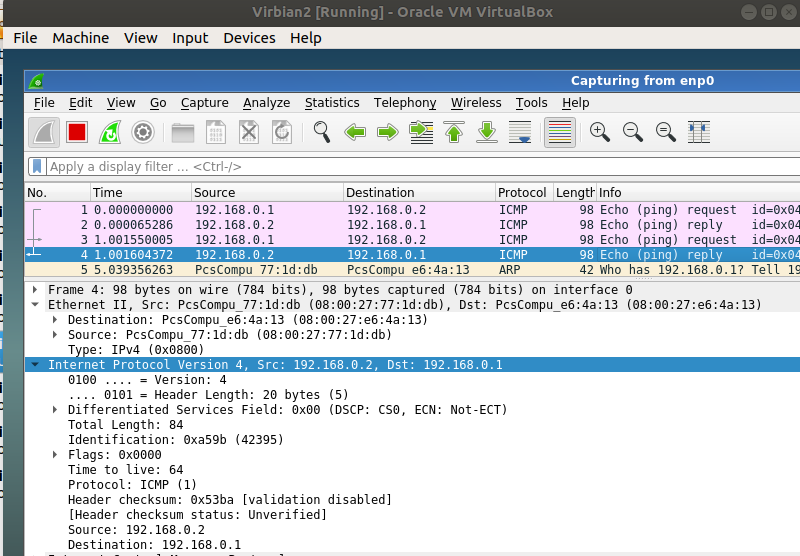
\includegraphics[width=11cm,height=5cm]{broadrep.png}
\caption{echo request}
\end{figure}
\tabto{0.4cm}Jakie są pola nadawcy i odbiorcy ramki ethernetowej? 
\tabto{0.8cm}Adresy MAC maszyn
\tabto{0.4cm}Jakie są pola nadawcy i odbiorcyzawartego w niej pakietu IP?
\tabto{0.8cm}Adresy IP maszyn.
\subsection{Ping -b 192.168.0.255}
\begin{figure}[!htb]
\centering
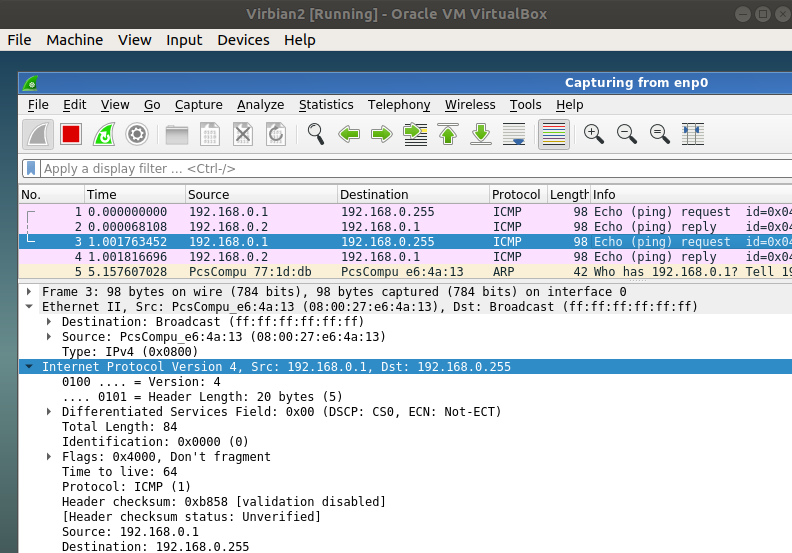
\includegraphics[width=11cm,height=5cm]{pingreq.png}
\caption{echo request}
\end{figure}
\begin{figure}[!htb]
\centering
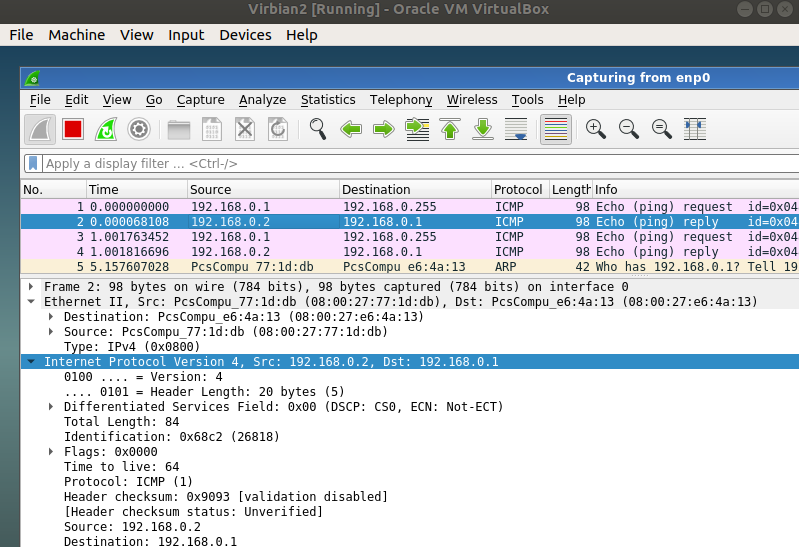
\includegraphics[width=11cm,height=5cm]{pingrep.png}
\caption{echo reply}
\end{figure}

\tabto{0.4cm}Jakie są pola nadawcy i odbiorcy ramki ethernetowej? 
\tabto{0.8cm}Adresy MAC maszyny dla nadawcy i rozgłoszeniowy w przypadku odbiorcy dla request, a  maszyn w przypadku reply.
\tabto{0.4cm}Jakie są pola nadawcy i odbiorcyzawartego w niej pakietu IP?
\tabto{0.8cm}Podobnie jak powyżej tylko dla adresów ip.
\newpage
\subsection{Tablica ARP}
\tabto{0.8cm}    ip neigh
\begin{figure}[!htb]
\centering
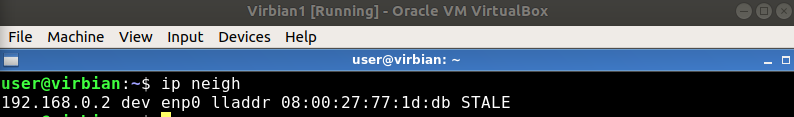
\includegraphics[width=11cm,height=1cm]{neighv1.png}
\caption{ip neigh dla V1}
\end{figure}
\begin{figure}[!htb]
\centering
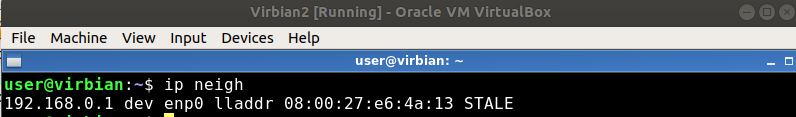
\includegraphics[width=11cm,height=1cm]{neighv2.png}
\caption{ip neigh dla V2}
\end{figure}
\tabto{0.8cm}    ip neigh flush all
\\
\tabto{0.4cm}Jak zmienił się stan tablicy ARP obu maszyn?
\tabto{0.8cm}Tablica zostaje wyczyszczona - pusta, ale po ping'u wraca do stanu sprzed wyczyszczeniem.
\subsection{Odpowiedzi}

\begin{figure}[!htb]
\centering
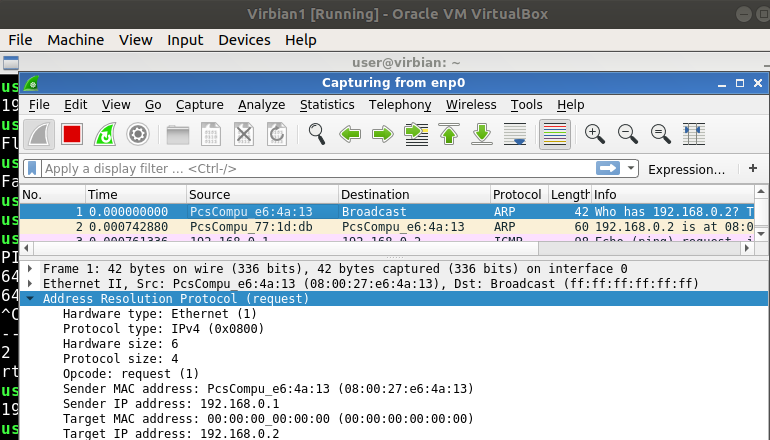
\includegraphics[width=11cm,height=5cm]{arpask.png}
\caption{ARP asking}
\end{figure}
\begin{figure}[!htb]
\centering
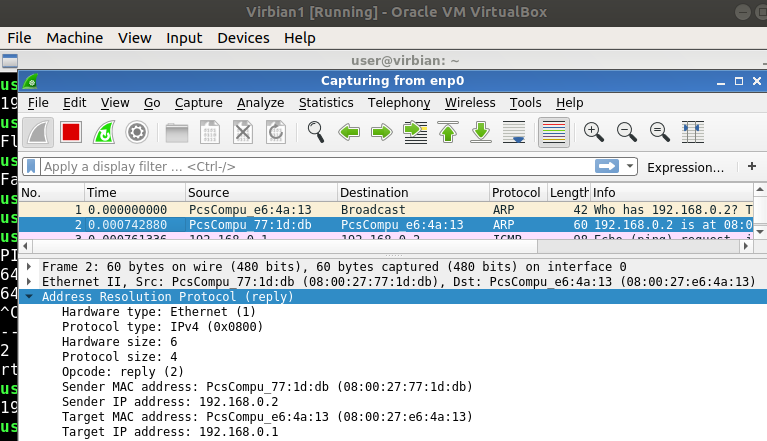
\includegraphics[width=11cm,height=5cm]{arprep.png}
\caption{ARP replying}
\end{figure}
\subsubsection{Co jest danymi ramki w przypadku zapytań ARP?} Danymi są np. adresy MAC oraz IP zarówno nadawcy jak i odbiorcy(target) adrec MAC odbiorcy przy zapytaniu jest wyzerowany, ponieważ go nie znamy.
\subsubsection{Czy zapytania ARP są wysyłane do konkretnego komputera czy na adres rozgłoszeniowy?}
Są wysyłane na adres rozgłoszeniowy.
\subsubsection{Czy odpowiedzi ARP są wysyłane do konkretnego komputera czy na adres rozgłoszeniowy?}
Odpowiedzi są wysyłane do komputera, z którego otrzymały zapytanie.

\section{Część 2.}
Sieć została skonfigurowana zgodnie z poleceniem.
\subsection{Jakie są zakresy adresów tych sieci?}
\tabto{0.4cm} V1 192.168.1.0/24 od 192.168.1.0 - 192.168.1.255
\tabto{0.4cm} V2 192.168.1.0/25 od 192.168.1.0 - 192.168.1.127
\tabto{0.4cm} V3 192.168.1.0/24 od 192.168.1.0 - 192.168.1.255
\tabto{0.4cm} V4 192.168.1.128/25 od 192.168.1.128 - 192.168.1.255
\subsection{Ping z V1}

\subsubsection{Które maszyny otrzymały komunikat ICMP echo request? Które nie otrzymały i dlaczego?}
Wszystkie maszyny.

\subsubsection{Które maszyny wysłały w odpowiedzi komunikat ICMP echo reply? Które nie wysłały i dlaczego?}
Tylko maszyna V3 wysłała odpowiedź, ponieważ ona należy do tej sieci. V4 nie wysłało, ponieważ adres V1 nie leży w zakresie adresów, a V2 nie wysłało opowiedzi, ponieważ to nie do niej był skierowany echo request (V2 podobnie będzie się zachowywało w innych podpunktach).

\subsubsection{Które odpowiedzi dotarły do maszyny Virbian1 ? Które nie dotarły i dlaczego?}
Tylko odpowiedź z maszyny V3 bo tylko ona wysłała oraz V1 było w "jej zasięgu".

\subsection{Ping z V2}

\subsubsection{Które maszyny otrzymały komunikat ICMP echo request? Które nie otrzymały i dlaczego?}
Wszystkie maszyny.

\subsubsection{Które maszyny wysłały w odpowiedzi komunikat ICMP echo reply? Które nie wysłały i dlaczego?}
Żadna maszyna nie wysłała odpowiedzi, ponieważ 192.168.1.127 dla innych maszyn nie jest adresem rozgłoszeniowym więc ją zignorowały.

\subsubsection{Które odpowiedzi dotarły do maszyny Virbian1 ? Które nie dotarły i dlaczego?}
Żadna odpowiedź nie dotarła.

\subsection{Ping z V3}

\subsubsection{Które maszyny otrzymały komunikat ICMP echo request? Które nie otrzymały i dlaczego?}
Wszystkie maszyny.

\subsubsection{Które maszyny wysłały w odpowiedzi komunikat ICMP echo reply? Które nie wysłały i dlaczego?}
Maszyna V1 i V4 wysłały odpowiedź, ponieważ dla obu maszyn jest to adres rozgłoszeniowy ich siec, mimo że są one w innych sieciach oraz adres V3 należy do ich sieci.

\subsubsection{Które odpowiedzi dotarły do maszyny Virbian1 ? Które nie dotarły i dlaczego?}
Wszystkie odpowiedzi dotarły.

\subsection{Ping z V4}

\subsubsection{Które maszyny otrzymały komunikat ICMP echo request? Które nie otrzymały i dlaczego?}
Wszystkie maszyny.

\subsubsection{Które maszyny wysłały w odpowiedzi komunikat ICMP echo reply? Które nie wysłały i dlaczego?}
Maszyna V1 i V3 wysłały odpowiedź, ponieważ dla obu maszyn jest to adres rozgłoszeniowy ich siec i adres V4 należy do ich sieci

\subsubsection{Które odpowiedzi dotarły do maszyny Virbian1 ? Które nie dotarły i dlaczego?}
Wszystkie dotarły.


\end{document}
